% Drawing 154/06-2 -- folder 154, batch 06, archive page 102 (PDF page 103).
% Transcription: page de dessins en couleur : plusieurs disques bordés de vert clair traversés de pseudo-droites orange, certains au crayon, quelques secteurs hachurés ou coloriés ; un petit disque partagé par un arc brun ; un demi-disque et un segment de disque traversés d'arcs orange. En bas à droite, un grand disque traversé de pseudo-droites orange et d'un faisceau de courbes vert clair qui le parcourent de haut en bas ; les points d'intersection sont marqués, et le bord porte, au crayon, des numéros (lus $1$, $2$, $8$, $9$, $11$, $15$, $16$, $18$, en partie incertains)
% Kind: several disks with arrangements; a large disk with a sweep and numbered rim. Method 2 (schematic redraw from the facsimile). Status: partial.
% Notes: Over typed notices of the computing centre (JESNEWS, Cadarache, Aug 1982; not reproduced). Several disks bordered in light green crossed by orange pseudolines, one in pencil, a few sectors hatched or coloured (left out); a small disk divided by a brown arc (the arc drawn orange-brown); a half-disk and a segment of disk crossed by orange arcs. Bottom right, a large disk crossed by orange pseudolines and by a pencil of light green curves running through it from top to bottom; the crossings are marked, and the rim carries pencil numbers (read 1, 2, 8, 9, 11, 15, 16, 18 in the transcription; placed here approximately, not re-read). Read from the page view; all arrangements are schematic.
% Coordinates: 1 unit = 1 mm = 1/100 of the crop width (bbox in page fractions: [0.42, 0.127, 0.964, 0.528]).
% Redrawn by Claude (claude-opus-5-5), issue #73, 2026-11-07; not checked by a human; not compiled (no TeX in the session).
% Rights: reproduces part of the work -- behind RENDER_TRANSCRIPTS, never published by itself.
\documentclass[tikz,border=3pt]{standalone}
\usepackage{amsmath,amssymb}
\usetikzlibrary{patterns,arrows.meta}
\tikzset{Or/.style={orange!90!black}, Ye/.style={yellow!80!orange}, Lg/.style={green!60!black!70}, Dg/.style={green!45!black}, Br/.style={brown!80!black}, Rd/.style={red!85!black}, Bl/.style={blue!70!black}, Gy/.style={black!40}, pencil/.style={black!45}, struck/.style={black!35}, mark/.style={circle,draw,inner sep=1.3pt}, pt/.style={circle,fill,inner sep=0.9pt}, opt/.style={circle,draw,fill=white,inner sep=1.1pt}}
\begin{document}
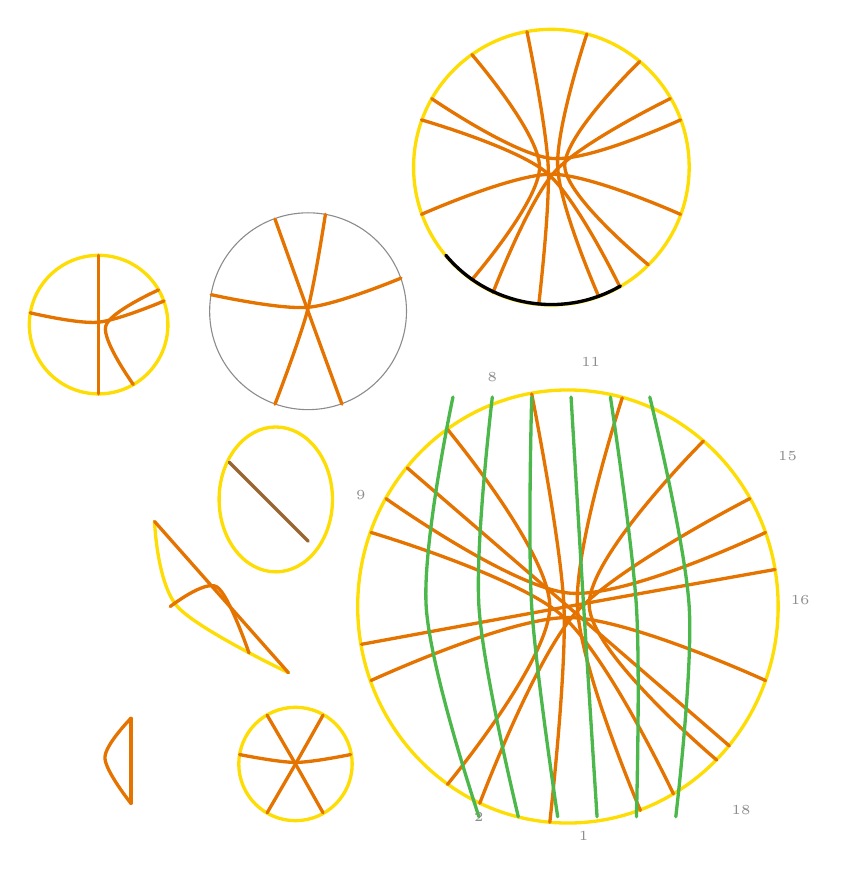
\begin{tikzpicture}[x=1mm,y=1mm,line cap=round,line join=round,font=\scriptsize]
\draw[Ye,very thick] (69.2,-20) ellipse[x radius=17.5, y radius=17.5];
\draw[Or,very thick] plot[smooth, tension=0.55] coordinates {(66.1,-2.8) (68.8,-20) (67.6,-37.4)};
\draw[Or,very thick] plot[smooth, tension=0.55] coordinates {(73.7,-3.1) (70,-20) (75.2,-36.4)};
\draw[Or,very thick] plot[smooth, tension=0.55] coordinates {(59.1,-5.7) (67.7,-20) (59.1,-34.3)};
\draw[Or,very thick] plot[smooth, tension=0.55] coordinates {(80.4,-6.6) (70.9,-19.9) (81.5,-32.4)};
\draw[Or,very thick] plot[smooth, tension=0.55] coordinates {(54,-11.3) (69.3,-18.9) (85.6,-14)};
\draw[Or,very thick] plot[smooth, tension=0.55] coordinates {(52.7,-26) (69.2,-20.9) (85.6,-26)};
\draw[Or,very thick] plot[smooth, tension=0.55] coordinates {(84.3,-11.3) (69.7,-20.5) (61.8,-35.9)};
\draw[Or,very thick] plot[smooth, tension=0.55] coordinates {(52.7,-14) (68.6,-20.7) (77.9,-35.2)};
\draw[very thick] (55.8,-31.2) arc[start angle=220, end angle=300, x radius=17.5, y radius=17.5];
\draw[pencil] (38.3,-38.3) circle[radius=12.5];
\draw[Or,very thick] plot[smooth, tension=0.55] coordinates {(40.5,-26) (38.2,-38.3) (34.1,-50.1)};
\draw[Or,very thick] plot[smooth, tension=0.55] coordinates {(34.1,-26.6) (38.3,-38.3) (42.6,-50.1)};
\draw[Or,very thick] plot[smooth, tension=0.55] coordinates {(26,-36.2) (38.3,-37.8) (50.1,-34.1)};
\draw[Ye,very thick] (11.7,-40) circle[radius=8.8];
\draw[Or,very thick] plot[smooth, tension=0.55] coordinates {(11.7,-31.2) (11.7,-40) (11.7,-48.8)};
\draw[Or,very thick] plot[smooth, tension=0.55] coordinates {(3,-38.5) (11.6,-39.7) (20,-37)};
\draw[Or,very thick] plot[smooth, tension=0.55] coordinates {(16.1,-47.6) (12.6,-40.2) (19.3,-35.6)};
\draw[Ye,very thick] (34.2,-62.2) ellipse[x radius=7.2, y radius=9.2];
\draw[Br,very thick] plot[smooth, tension=0.55] coordinates {(28.3,-57.5) (33.3,-62.5) (38.3,-67.5)};
\draw[Ye,very thick] plot[smooth, tension=0.55] coordinates {(18.8,-65) (21.7,-75.8) (35.8,-84.2)};
\draw[Or,very thick] (18.8,-65) -- (35.8,-84.2);
\draw[Or,very thick] plot[smooth, tension=0.55] coordinates {(20.8,-75.8) (26.7,-73.3) (30.8,-81.7)};
\draw[Ye,very thick] (36.7,-95.8) circle[radius=7.2];
\draw[Or,very thick] plot[smooth, tension=0.55] coordinates {(40.2,-89.6) (36.7,-95.8) (33.1,-102)};
\draw[Or,very thick] plot[smooth, tension=0.55] coordinates {(33.1,-89.6) (36.7,-95.8) (40.2,-102)};
\draw[Or,very thick] plot[smooth, tension=0.55] coordinates {(29.6,-94.6) (36.7,-95.6) (43.7,-94.6)};
\draw[Or,very thick] plot[smooth, tension=0.55] coordinates {(15.8,-90) (12.5,-95) (15.8,-100.8)};
\draw[Or,very thick] (15.8,-90) -- (15.8,-100.8);
\draw[Ye,very thick] (71.3,-75.8) ellipse[x radius=26.7, y radius=27.5];
\draw[Or,very thick] plot[smooth, tension=0.55] coordinates {(66.7,-48.8) (70.8,-75.9) (69,-103.2)};
\draw[Or,very thick] plot[smooth, tension=0.55] coordinates {(78.2,-49.3) (72.5,-75.8) (80.5,-101.7)};
\draw[Or,very thick] plot[smooth, tension=0.55] coordinates {(56,-53.3) (69,-75.8) (56,-98.4)};
\draw[Or,very thick] plot[smooth, tension=0.55] coordinates {(88.5,-54.8) (74,-75.7) (90.2,-95.3)};
\draw[Or,very thick] plot[smooth, tension=0.55] coordinates {(48.2,-62.1) (71.5,-74.1) (96.4,-66.4)};
\draw[Or,very thick] plot[smooth, tension=0.55] coordinates {(46.3,-85.2) (71.3,-77.2) (96.4,-85.2)};
\draw[Or,very thick] plot[smooth, tension=0.55] coordinates {(94.4,-62.1) (72.2,-76.7) (60.1,-100.8)};
\draw[Or,very thick] plot[smooth, tension=0.55] coordinates {(46.3,-66.4) (70.5,-76.9) (84.7,-99.6)};
\draw[Or,very thick] plot[smooth, tension=0.55] coordinates {(97.6,-71.1) (71.3,-75.8) (45.1,-80.6)};
\draw[Or,very thick] plot[smooth, tension=0.55] coordinates {(50.9,-58.2) (71.3,-75.8) (91.8,-93.5)};
\draw[Lg,very thick] plot[smooth, tension=0.55] coordinates {(56.7,-49.2) (53.3,-75.8) (60,-102.5)};
\draw[Lg,very thick] plot[smooth, tension=0.55] coordinates {(61.7,-49.2) (60,-75.8) (65,-102.5)};
\draw[Lg,very thick] plot[smooth, tension=0.55] coordinates {(66.7,-49.2) (66.7,-75.8) (70,-102.5)};
\draw[Lg,very thick] plot[smooth, tension=0.55] coordinates {(71.7,-49.2) (73.3,-75.8) (75,-102.5)};
\draw[Lg,very thick] plot[smooth, tension=0.55] coordinates {(76.7,-49.2) (80,-75.8) (80,-102.5)};
\draw[Lg,very thick] plot[smooth, tension=0.55] coordinates {(81.7,-49.2) (86.7,-75.8) (85,-102.5)};
\node[inner sep=1pt,pencil] at (73.3,-105) {\tiny $1$};
\node[inner sep=1pt,pencil] at (60,-102.5) {\tiny $2$};
\node[inner sep=1pt,pencil] at (61.7,-46.7) {\tiny $8$};
\node[inner sep=1pt,pencil] at (45,-61.7) {\tiny $9$};
\node[inner sep=1pt,pencil] at (74.2,-44.7) {\tiny $11$};
\node[inner sep=1pt,pencil] at (99.2,-56.7) {\tiny $15$};
\node[inner sep=1pt,pencil] at (100.8,-75) {\tiny $16$};
\node[inner sep=1pt,pencil] at (93.3,-101.7) {\tiny $18$};
\end{tikzpicture}
\end{document}
